\section*{Metode}
\label{Metode}
%
%What type of MDS should you use? Argue for choice
Indenfor \textit{Multidimensional scaling (MDS)} findes der tre standard metoder, der kan anvendes, herunder \textit{Classical MDS}, \textit{Non-classical MDS} og \textit{Non-metric MDS}. For at bestemme hvilken af de tre metoder, der bør anvendes, skal det vurderes, om data i datasættet er interval eller ordinal data. Derefter vurderes det om der ønskes at bruge en metode, som anvender lineær algebra eller iterative algoritmer, til finde den optimale løsning. 

Til analysen i denne rapport vælges det at anvende metoden \textit{Non-metric MDS}, da datasættet består af ordinal data. Metoden passer til datasættet, da den kun kræver denne type data, hvor interval og ratio information er ikke relevant for denne metode \parencite[p.9]{Wickelmaier2003}. 
\\\\
Ved MDS skal antallet af dimensioner bestemmes. Til at tolke hvor godt det valgte antal dimensioner passer på ens data bruges begrebet \textit{stress}, som er et udtryk for godt de reelle forskelle er præsenteret. 

Ved bestemmelse af antal dimensioner er det en vurdering mellem hvor let det skal være at fortolke og hvor lidt stress der skal være. Jo flere dimensioner der vælges, jo sværre vil det være at fortolke skalaen, men samtidig vil der være mindre stress. På \autoref{fig:TolkningStress} kan sammenhængen mellem stress værdien og hvor godt fit'et er, aflæses. 

\begin{figure}[H]
\centering
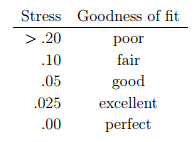
\includegraphics[width = 0.25\textwidth]{Figure/TolkningStress.PNG} 
\caption{Fortolkning af stress i forhold til hvor godt et fit antallet af dimensioner er \parencite[p.13]{Wickelmaier2003}. }
\label{fig:TolkningStress}
\end{figure}
